\begin{section}{Results}

A simultaneous fit to the signal region across the three event categories, allowing for sytematic uncertainty variations of the background expectations, is performed.
The corresponding comparisons between data and background in the \ETm distributions, for each of the three categories, after this fit are shown in Figure~\ref{fig:post_fit_plots}.   
Agreement between the expected SM backgrounds and data is observed at the percent level across the three categories. The largest single-bin local significance across the three categories, is 1.9$\sigma$ and corresponds to the excess seen in the last \ETm bin of the monojet category.

\begin{figure*}[hbtp]\begin{center}
  \subfloat[][]{
 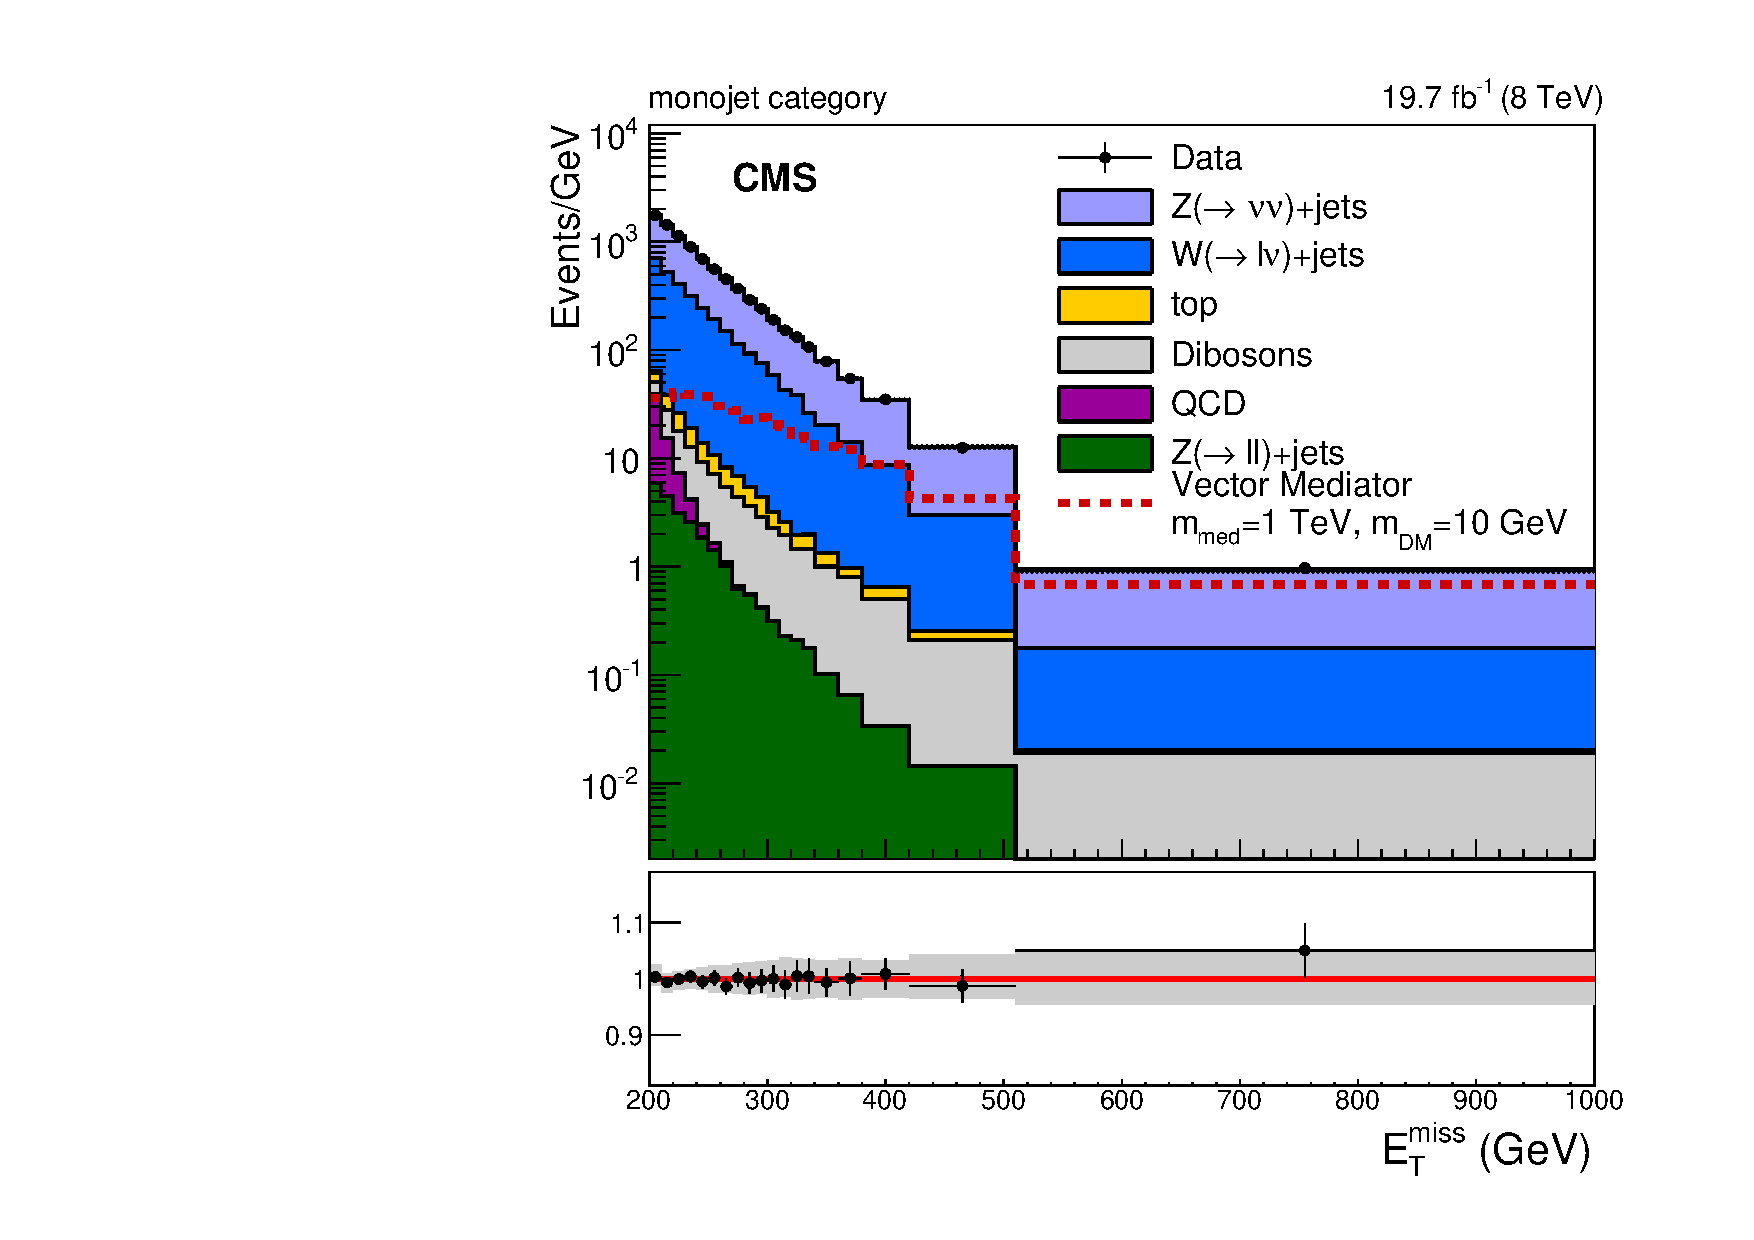
\includegraphics[width=0.5\textwidth]{figures/plot_config_monojet.pdf}
}
  \subfloat[][]{
 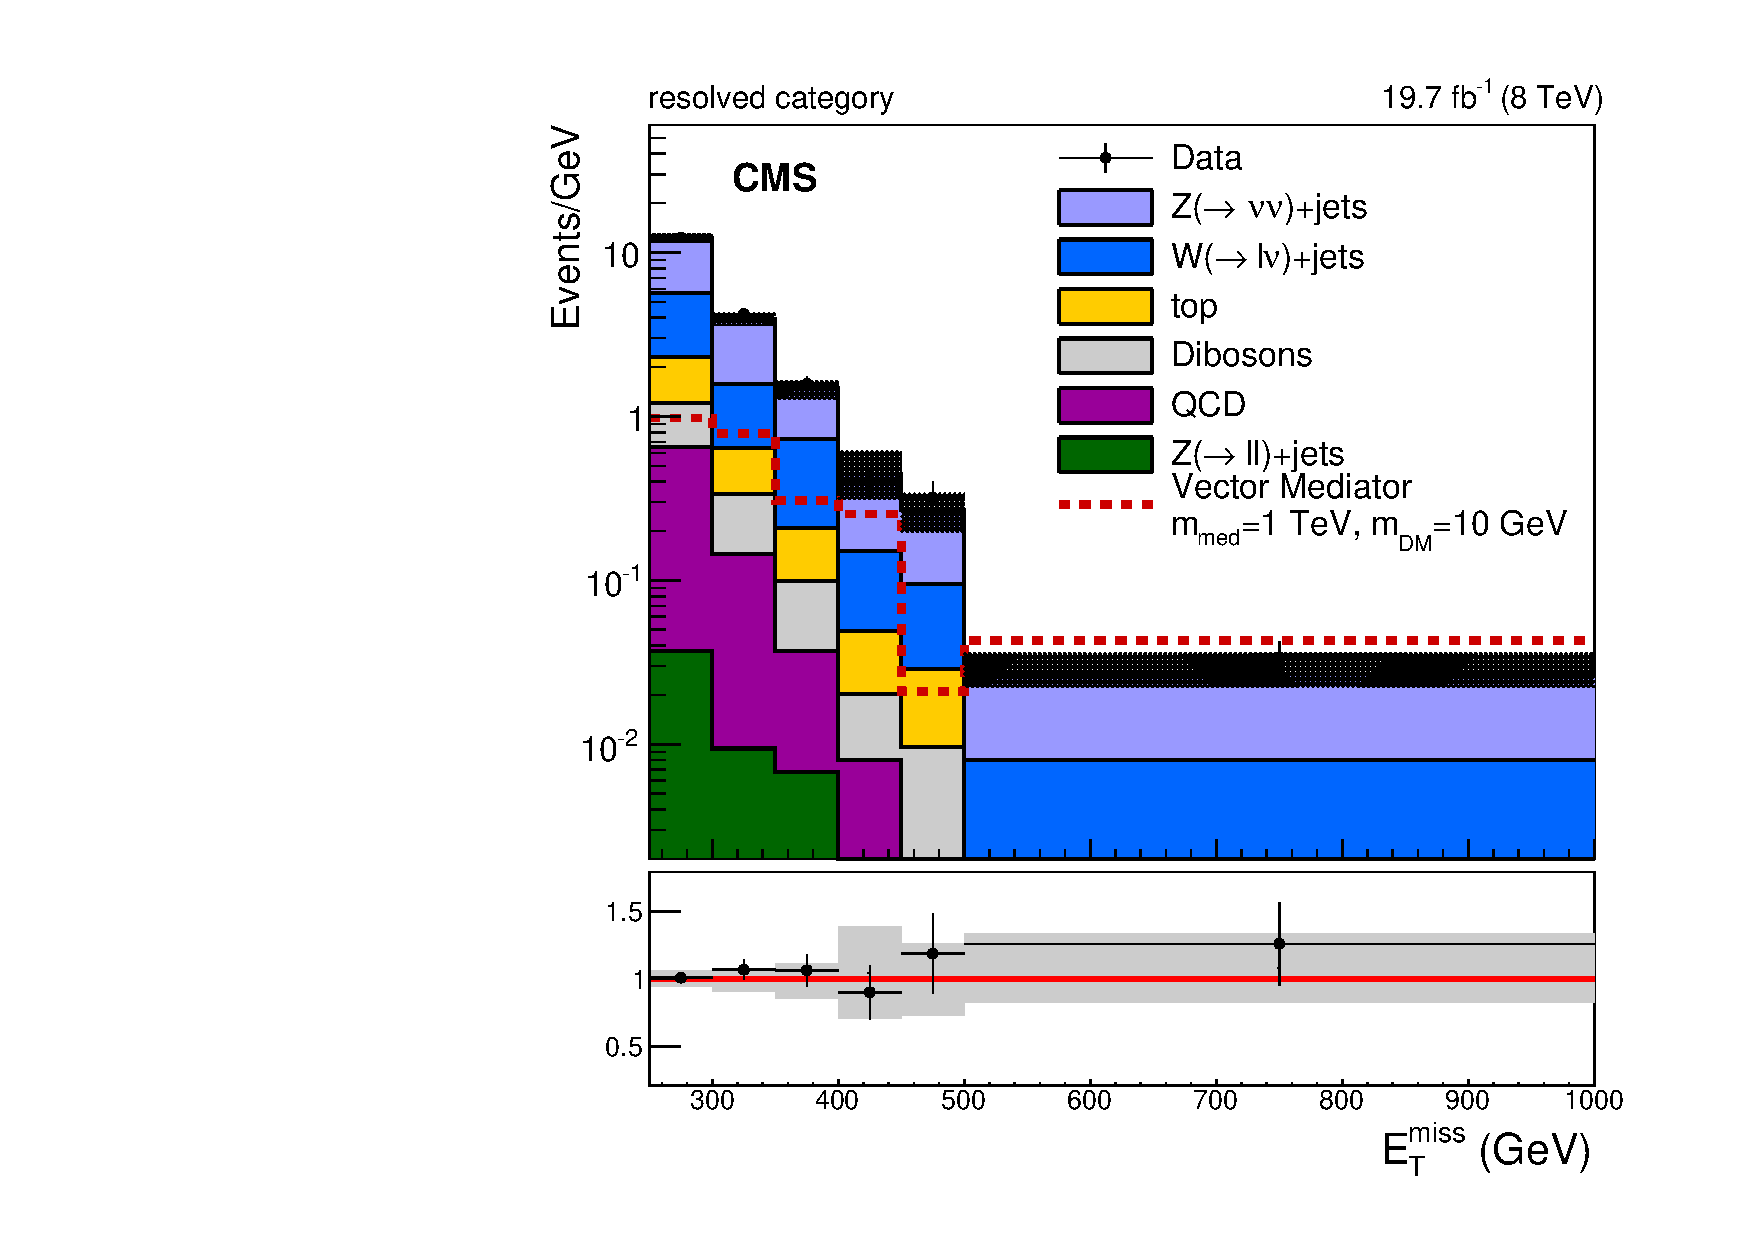
\includegraphics[width=0.5\textwidth]{figures/plot_config_resolved.pdf}
}\\
  \subfloat[][]{
 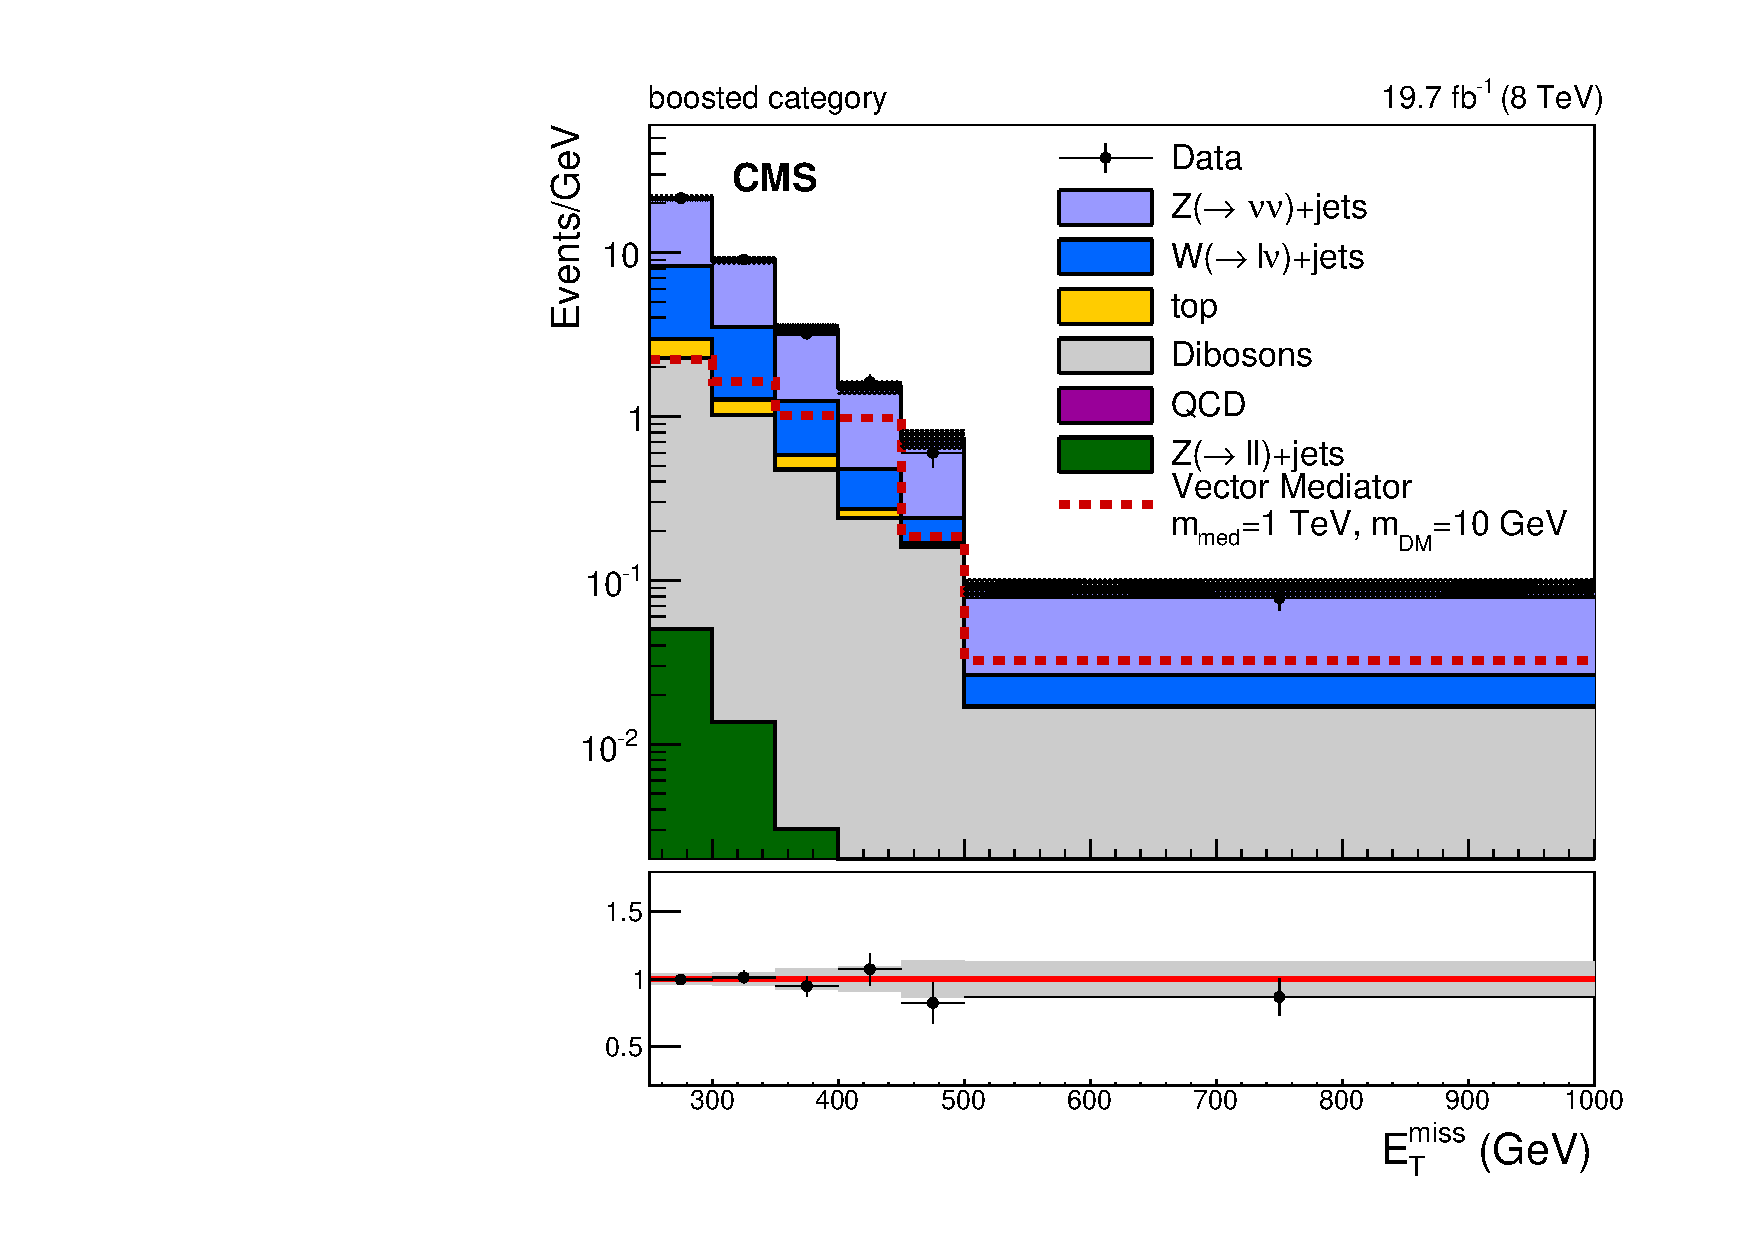
\includegraphics[width=0.5\textwidth]{figures/plot_config_boosted.pdf}
}
 \caption{
   Post-fit distributions of \ETm expected from SM backgrounds and observed in data in the signal region. The expected distributions are 
   evaluated after fitting to the observed data simultaneously across the monojet (a), resolved (b) and boosted (c) categories. 
   The gray bands indicate the post-fit uncertainty on the background, assuming no signal. The expected distribution assuming vector mediated DM production 
   is shown for a DM mass of 10 GeV and a mediator mass of 1 TeV.
 }
 \label{fig:post_fit_plots}\end{center}\end{figure*}

Exclusion limits are set for a number of DM models. The limits are calculated using the CLs method~\cite{cls} with a profile likelihood ratio as the 
test-statistic in which systematic uncertainties are modelled as nuisance parameters. 
For each signal hypothesis tested, upper limits are placed on the ratio of 
the signal cross-section to the predicted cross-section, denoted as $\mu=\sigma/\sigma_{TH}$. Limits are presented in terms of excluded regions in the 
$m_{\mathrm{MED}}-m_{\textrm{DM}}$ plane, assuming the four different mediators, by determining the points for which $\mu\ge1$ is excluded at 90\% CL or more.
Experimental systematic uncertainties, including jet and \ETm response and resolution, are included on the signal model as nuisance parameters, while the
theoretical systematic uncertainties on the inclusive cross-section (20\% and 30\% for the vector and axial-vector, and scalar and pseudoscalar models respectively) due to QCD scale and 
PDF uncertainties are instead added as additional contours to the exclusion limits. These uncertainties are chosen to be conservative across the full range in mediator mass.


To compare direct detection experiments with collider experiments, the direct detection bounds can be interpreted under the Lagrangians given in Equation~\ref{eq:LS}. The limits obtained in 
the simplified models are obtained using the standard approaches to compute t-channel scattering~\cite{Kurylov:2003ra,Hisano:2010ct, Cheung:2013pfa}. 
For the vector and scalar mediator models, the limits are compared with the measurements by LUX~\cite{Akerib:2012ys,Akerib:2013tjd,Szydagis:2014xog} which currently 
provides the strongest bounds for $m_{\rm DM} \gtrsim 6$ GeV. For axial-vector couplings, the limits are compared with the combined bounds 
of DM-proton-scattering limits of PICASSO \cite{Archambault:2012pm}, COUPP \cite{Behnke:2012ys} and SIMPLE \cite{Felizardo:2011uw}, while for the pseudoscalar case, the comparison is made 
with constraints from FermiLAT~\cite{Ackermann:2011wa,Abdo:2010ex}.
For pseudoscalar interactions, direct detection bounds are strongly velocity suppressed. 
The most appropriate comparison is therefore to the most sensitive bounds from indirect detection from FermiLAT. 
These limits apply to the scenario in which dark matter is annihilated in the center of a galaxy producing a $\gamma$ ray signature. 
The results are also compared, for all four types of mediators, to constraints obtained from the observed cosmological relic density of DM as determined from 
measurements of the cosmic microwave background by the WMAP and Planck experiments~\cite{Bennett:2003ba,Planck:2006aa}. The expected DM abundance is estimated, separately for each
model, using a thermal freeze-out mechanism implemented in MadDM~\cite{Backovic:2013dpa}, and compared to the observed cold DM density $\Omega_c*h^2=0.12$~\cite{Ade:2013zuv}. 
It is assumed that the simplified model hypothesised provides the only relevant BSM dynamics for DM interactions.

Figure~\ref{fig:masslims} shows the 90\% CL exclusions for the vector, axial-vector, 
scalar and pseudoscalar mediator models.  The 90\% confidence level upper limit on the ratio of excluded cross-section to the predicted cross-section ($\mu_{up}$), when assuming the mediator only 
couples to fermions, is shown by the blue color scale. These limits are conservative given the assumption that only the initial state partons and the DM 
particle contribute to the width of the mediator. For all models, the width is fixed under the minimum width constraint. For the vector 
mediator, the direct-detection bounds dominate above $m_{DM}=6$~\GeV, while for the axial-vector, scalar, pseudoscalar mediator models, the bounds 
from this analysis dominate over the whole region. 

\begin{figure}[htbp]
  \centering
  \subfloat[][]{
	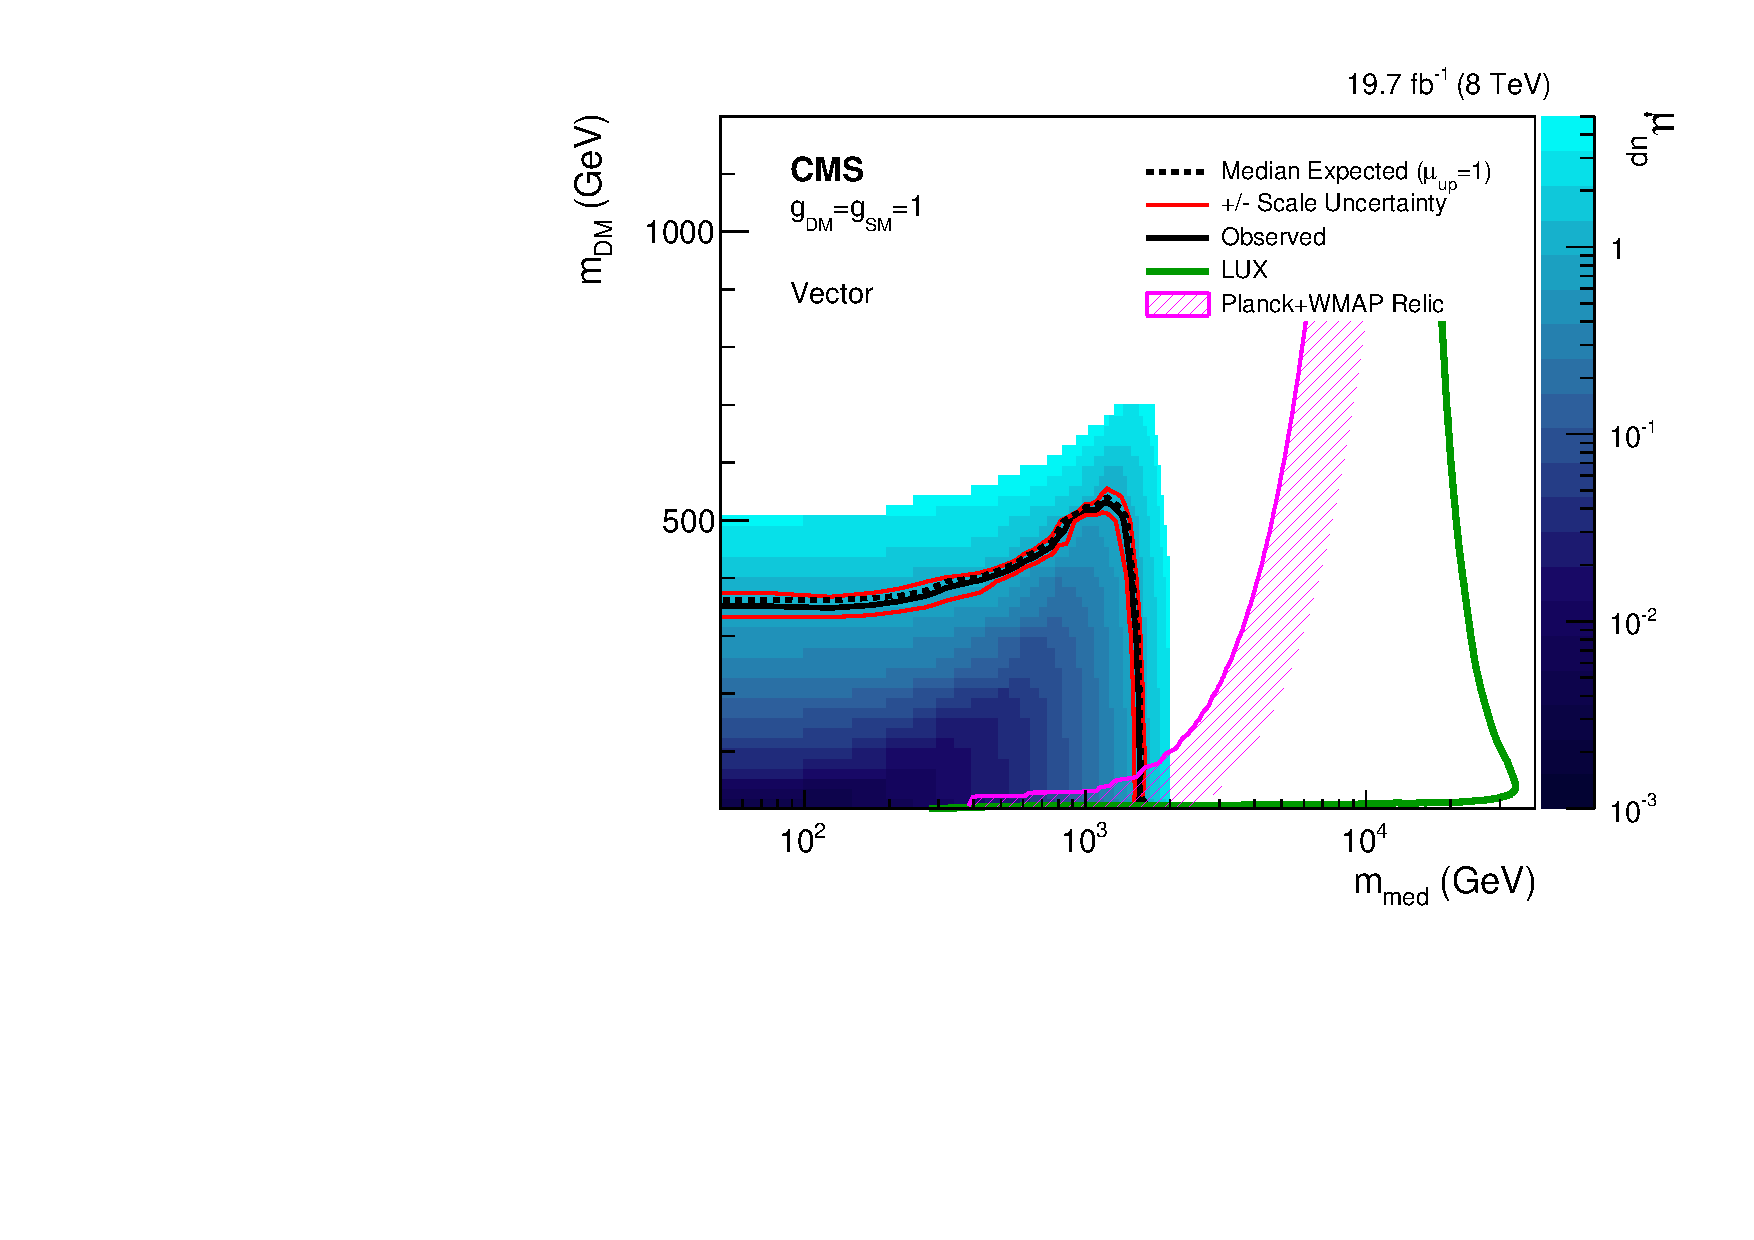
\includegraphics[angle=0,width=0.50\textwidth]{figures/MassLimit_1_800_0_Both.pdf}
	\label{fig:mass_800}
  }
  \subfloat[][]{
	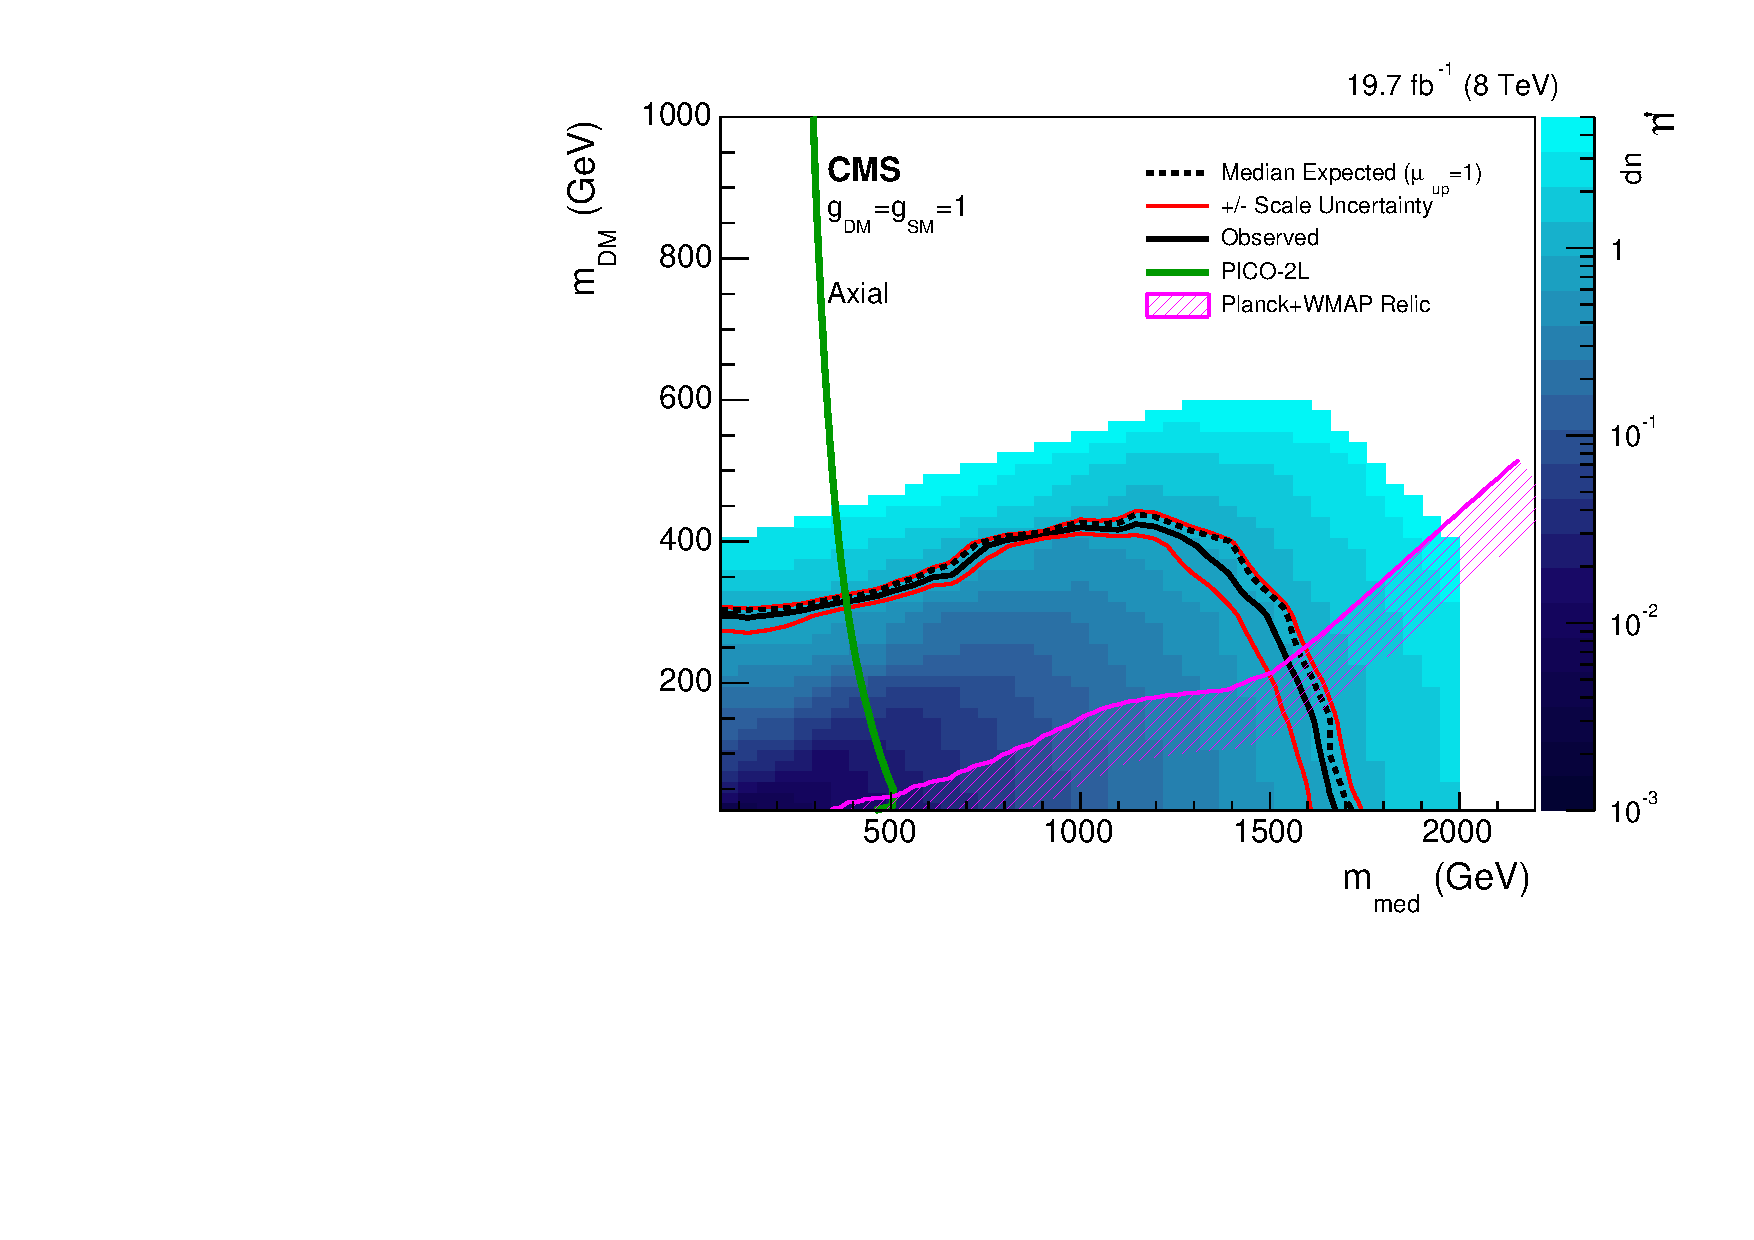
\includegraphics[angle=0,width=0.50\textwidth]{figures/MassLimit_1_801_0_Both.pdf}
	\label{fig:mass_801}
  }\\
  \subfloat[][]{
	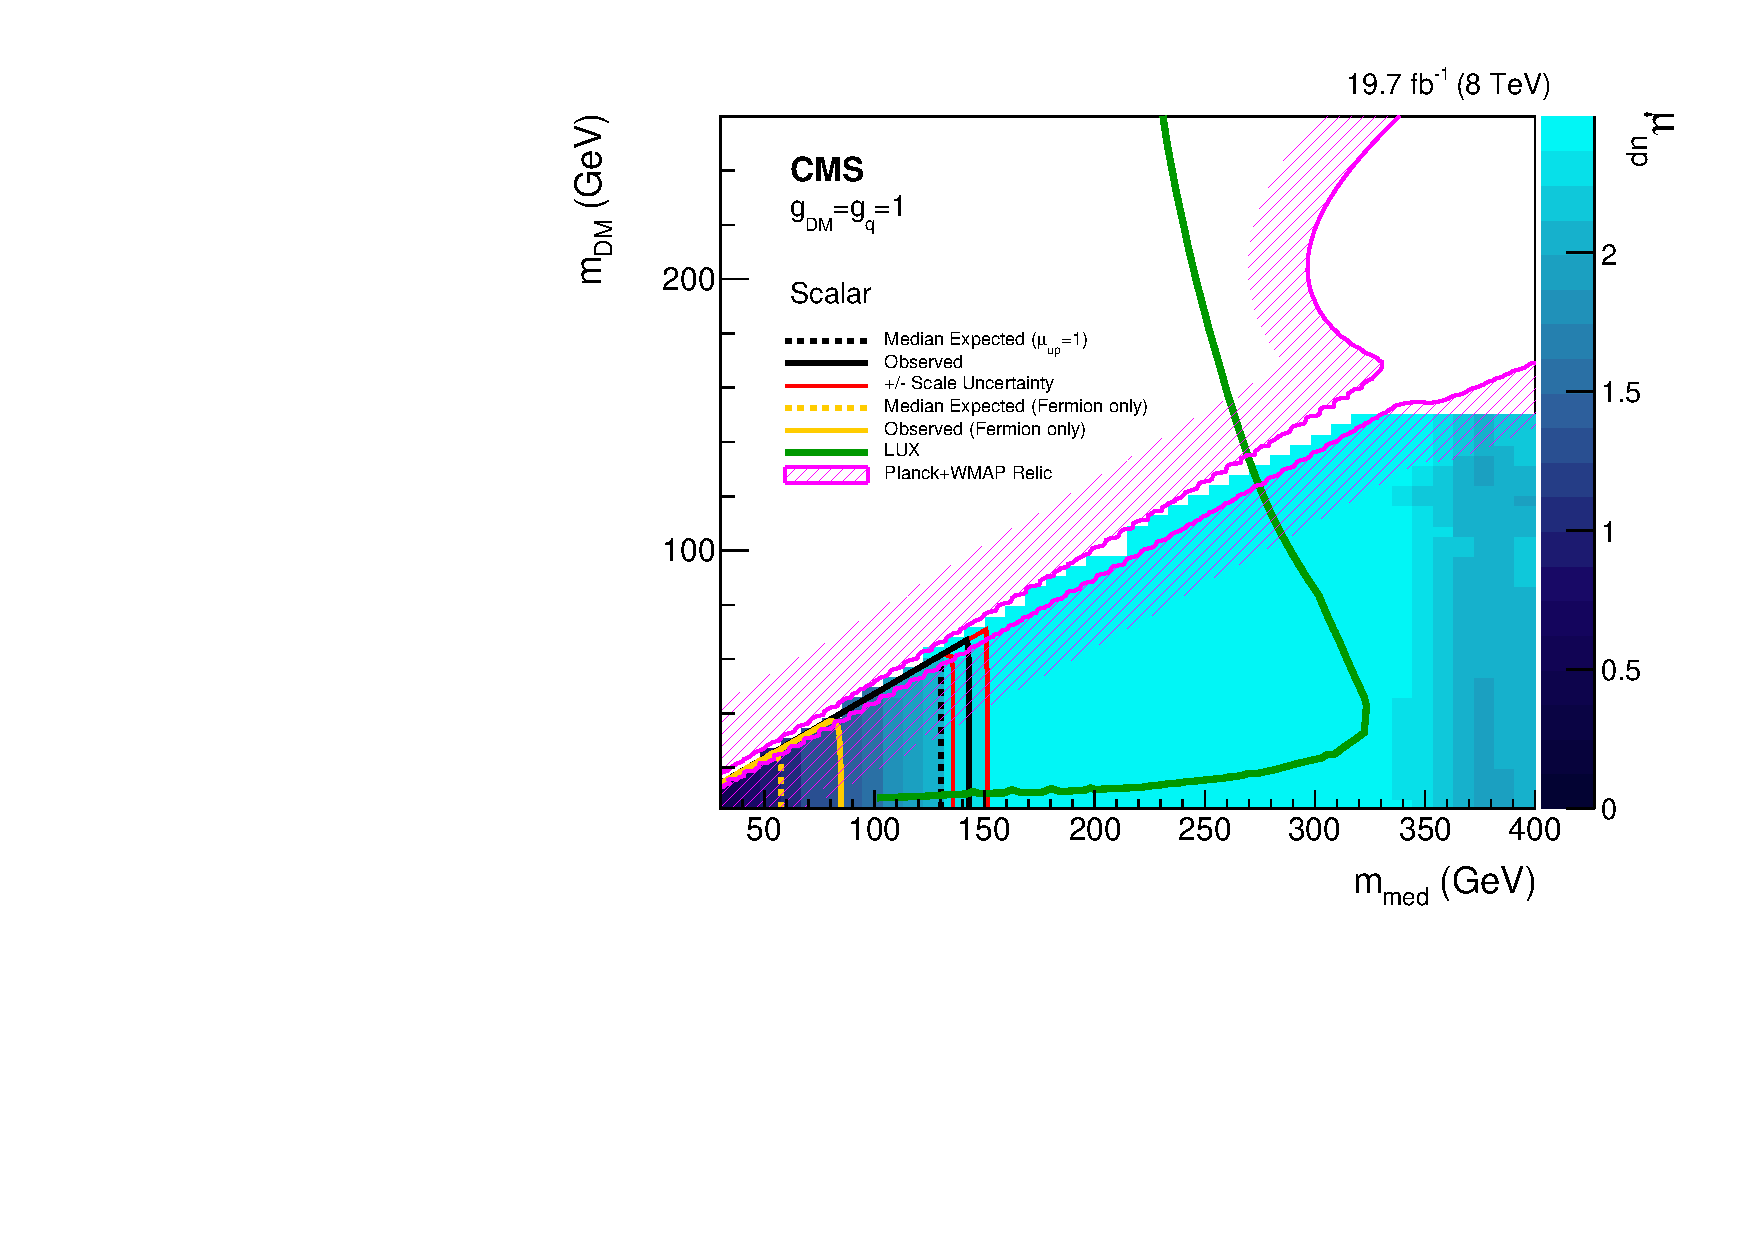
\includegraphics[angle=0,width=0.50\textwidth]{figures/MassLimit_1_805_0_Both.pdf}
	\label{fig:mass_805}
  }
  \subfloat[][]{
	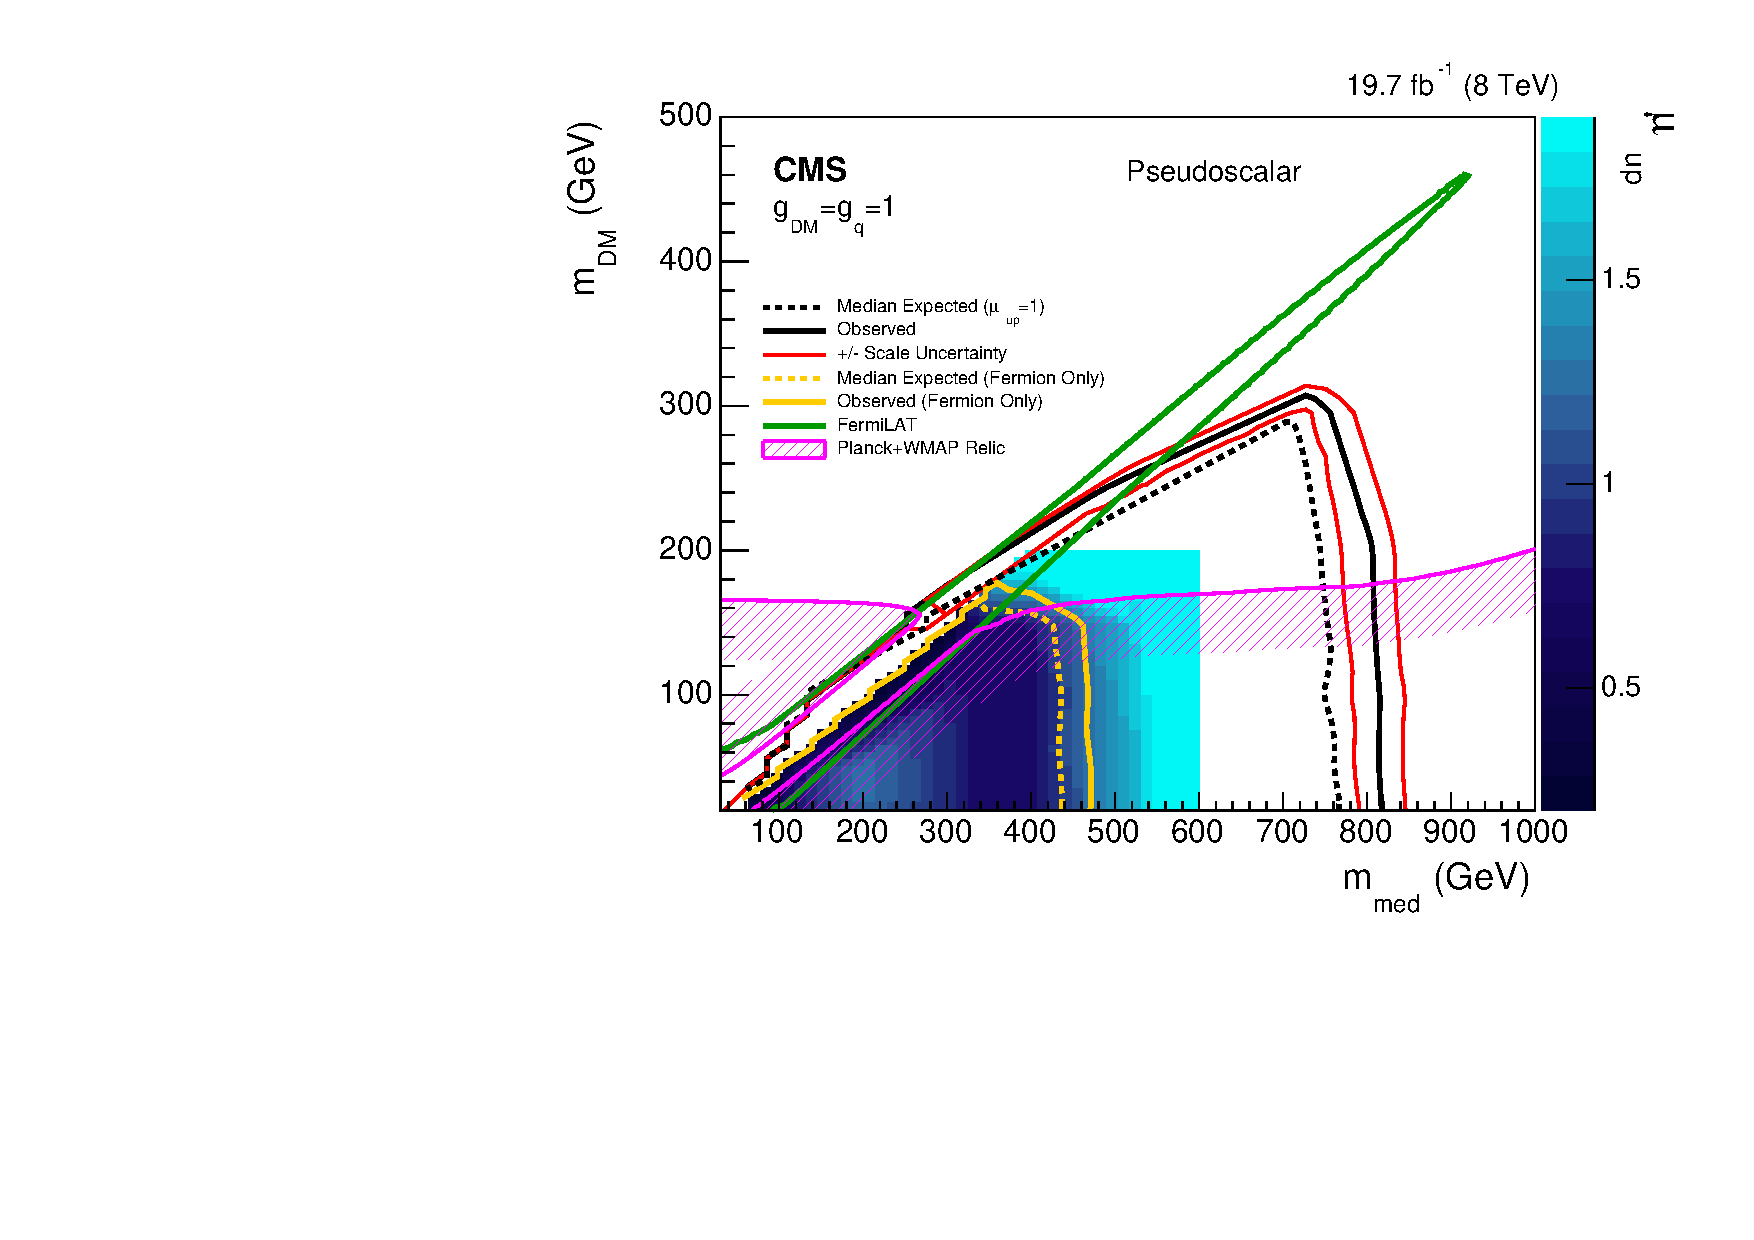
\includegraphics[angle=0,width=0.50\textwidth]{figures/MassLimit_1_806_0_Both.pdf}
	\label{fig:mass_806}
  }
  \caption{90\% CL Exclusion contours in the $m_{\textrm{med}}-m_{\textrm{DM}}$ plane assuming a vector (a), axial-vector (b), scalar (c), or pseudoscalar (d) mediator. 
The blue scale shows the 90\% CL upper limit on the signal strength assuming the mediator only couples to fermions. 
The excluded region is to the bottom-left of the contours shown in all cases except for that from the relic density as indicated by the shading.
In all of the mediator models, a minimum width is assumed\label{fig:masslims}.}
\end{figure}


%Figures~\ref{fig:xslims_800},~\ref{fig:xslims_801} and~\ref{fig:xslims_805} show the same exclusion contours, this time translated into the 
%plane of $m_{\textrm{DM}}-\sigma_{\textrm{DD}}$, where $\sigma_{\textrm{DM}}$ is 
%the spin-independent/dependant (vector and scalar/axial-vector) DM-nucleon scattering cross-section. 
%These representations allow for a more direct comparison with the direct-detection expedients which typically set 
%model-independent limits on these cross-sections. It should be noted that the limits set from this 
%analysis are however only valid under the simplified model considered, and in particular 
%assuming $g_{DM}=g_{SM}=1$. For the scalar model, it is assumed that only heavy quarks 
%(top and bottom) contribute. Such a choice limits the sensitivity for direct 
%detection, however it allows for direct comparison between collider and direct detection without an additional assumptions 

%on the light quark couplings~\cite{Harris:2015kda}.
 
Recent excesses observed in FermiLAT data have led to speculations that dark matter annihilation is mediated by a light pseudoscalar~\cite{Calore:2014nla}. 
The production mechanism for these $\gamma$ rays can be interpreted under dark matter annihilation to b-quarks allowing for direct 
comparison limits from this analysis~\cite{Harris:2014hga,Buckley:2014fba,Buchmueller:2013dya}. Figure~\ref{fig:xslims_806} shows 
the exclusion contours assuming pseudoscalar mediation in the plane of DM pair annihilation cross-section versus $m_{\textrm{DM}}$. 
It is assumed that only heavy quarks (top and bottom quarks) contribute. Such a choice limits the sensitivity for direct 
detection, however it allows for direct comparison between collider and direct detection without an additional assumptions 
on the light quark couplings~\cite{Harris:2015kda}.
The 68\% CL preferred regions in this plane assuming the annihilation of DM pairs to light-quarks (qq), tau or bottom pairs, using data from FermiLAT, 
are shown as solid colour regions. Under the simplified model used, all of these regions are excluded by this analysis.

\begin{figure}[htbp]
  \centering
	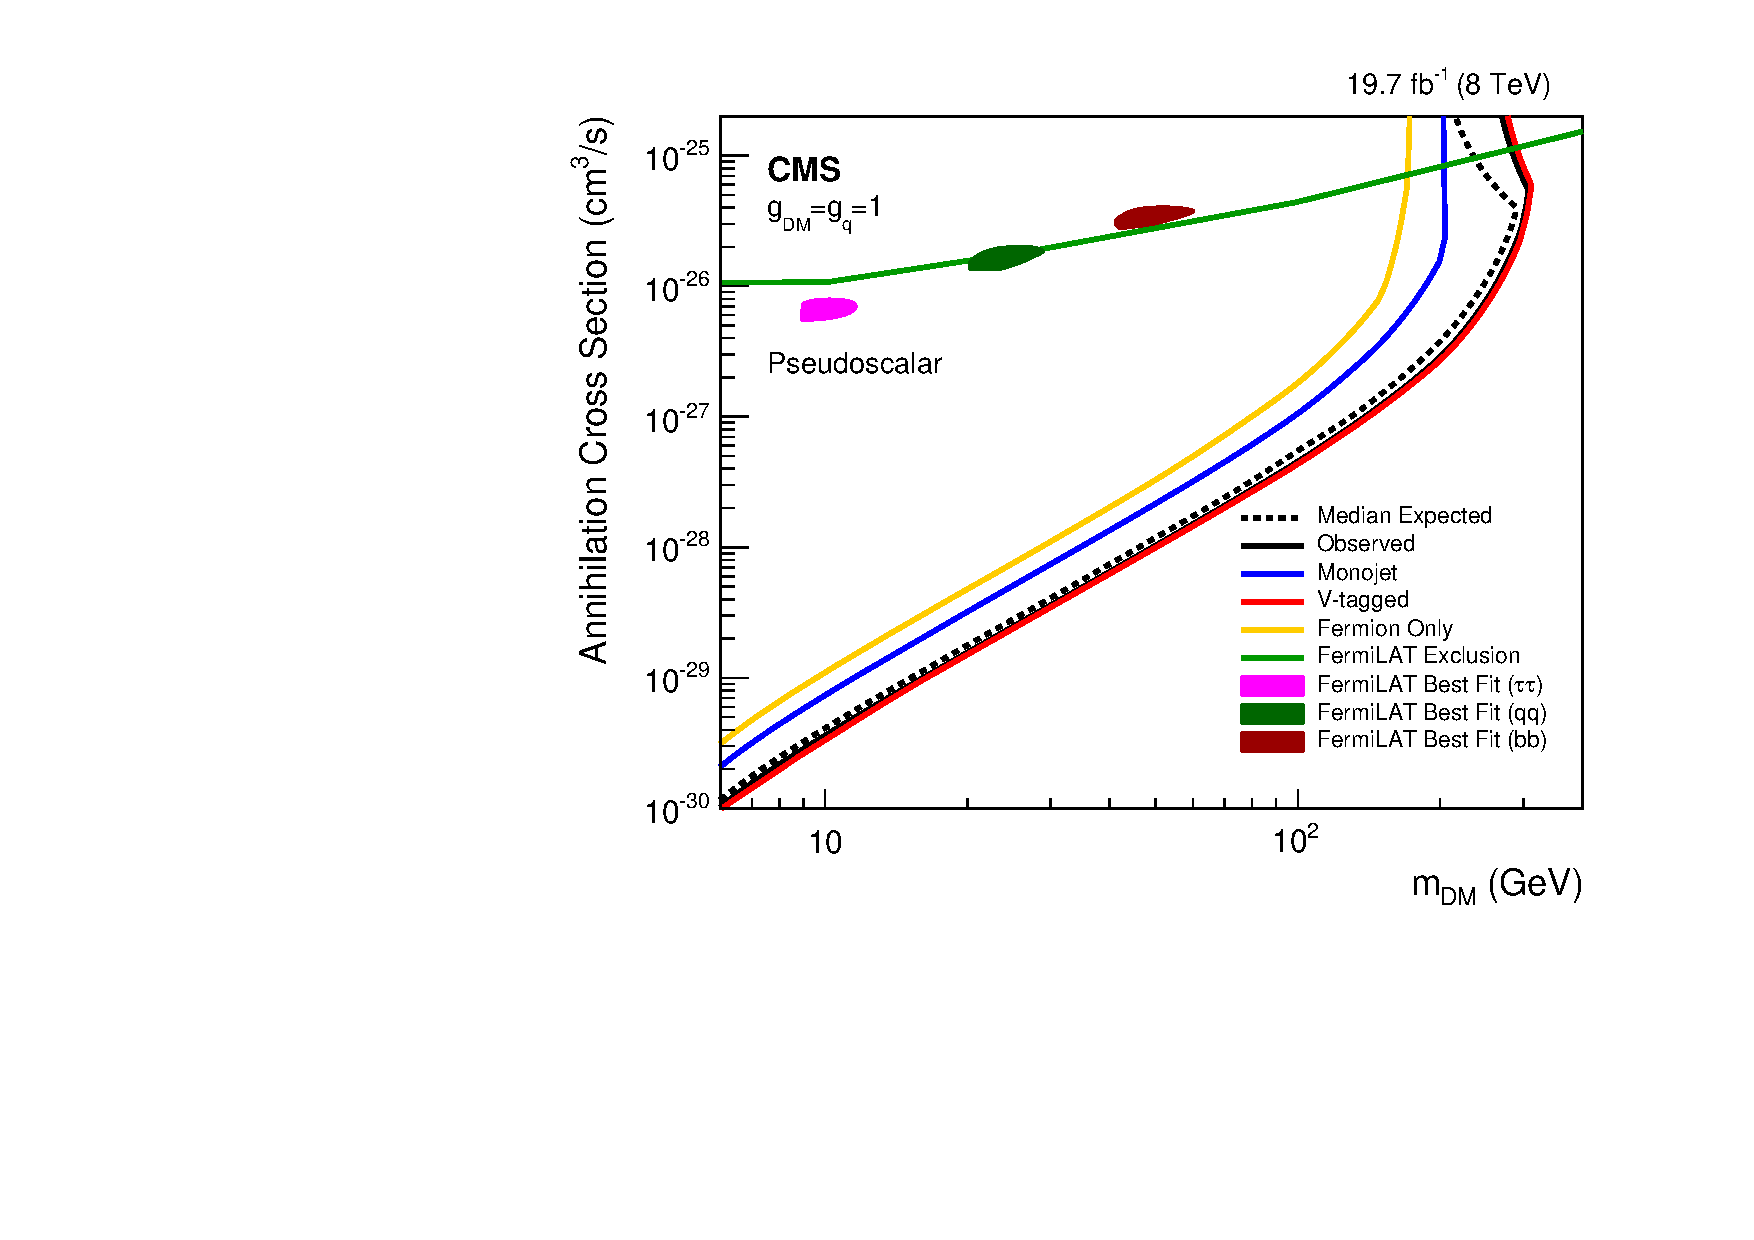
\includegraphics[angle=0,width=0.70\textwidth]{figures/MassLimit_1_806_0_Both_DD.pdf}
  \caption{90\% CL Exclusion contours in the $m_{\textrm{med}}-\sigma_{\textrm{DM}}$ plane assuming a pseudoscalar mediator. 
The orange line shows the exclusion contours assuming the mediator only couples to fermions. 68\% CL preferred regions, using data from FermiLAT, for DM annihilation 
to light-quarks (qq), tau pairs ($\tau\tau$) and bottom-quark pairs (bb) are shown by the solid green, pink and brown coloured regions respectively.\label{fig:xslims}}
\end{figure}


